\documentclass[14pt]{extbook}
\usepackage{multicol, enumerate, enumitem, hyperref, color, soul, setspace, parskip, fancyhdr} %General Packages
\usepackage{amssymb, amsthm, amsmath, bbm, latexsym, units, mathtools} %Math Packages
\everymath{\displaystyle} %All math in Display Style
% Packages with additional options
\usepackage[headsep=0.5cm,headheight=12pt, left=1 in,right= 1 in,top= 1 in,bottom= 1 in]{geometry}
\usepackage[usenames,dvipsnames]{xcolor}
\usepackage{dashrule}  % Package to use the command below to create lines between items
\newcommand{\litem}[1]{\item#1\hspace*{-1cm}\rule{\textwidth}{0.4pt}}
\pagestyle{fancy}
\lhead{Progress Quiz 4}
\chead{}
\rhead{Version C}
\lfoot{8448-1521}
\cfoot{}
\rfoot{Fall 2020}
\begin{document}

\begin{enumerate}
\litem{
Determine the domain of the function below.\[ f(x) = \frac{4}{24x^{2} -54 x + 30} \]\begin{enumerate}[label=\Alph*.]
\item \( \text{All Real numbers.} \)
\item \( \text{All Real numbers except } x = a, \text{ where } a \in [19.76, 20.41] \)
\item \( \text{All Real numbers except } x = a \text{ and } x = b, \text{ where } a \in [19.76, 20.41] \text{ and } b \in [34.9, 36.59] \)
\item \( \text{All Real numbers except } x = a \text{ and } x = b, \text{ where } a \in [0.39, 1.05] \text{ and } b \in [1.12, 1.67] \)
\item \( \text{All Real numbers except } x = a, \text{ where } a \in [0.39, 1.05] \)

\end{enumerate} }
\litem{
Solve the rational equation below. Then, choose the interval(s) that the solution(s) belongs to.\[ \frac{-4x}{-3x -7} + \frac{-2x^{2}}{15x^{2} +56 x + 49} = \frac{-7}{-5x -7} \]\begin{enumerate}[label=\Alph*.]
\item \( x_1 \in [1.34, 1.76] \text{ and } x_2 \in [-2.21,-1.38] \)
\item \( \text{All solutions lead to invalid or complex values in the equation.} \)
\item \( x_1 \in [1.34, 1.76] \text{ and } x_2 \in [-2.48,-2.09] \)
\item \( x \in [-2.4,-1.65] \)
\item \( x \in [-1.44,-1.29] \)

\end{enumerate} }
\litem{
Solve the rational equation below. Then, choose the interval(s) that the solution(s) belongs to.\[ \frac{-6}{-3x + 2} + 7 = \frac{4}{9x -6} \]\begin{enumerate}[label=\Alph*.]
\item \( x_1 \in [-1.27, -0.51] \text{ and } x_2 \in [-0.56,2.44] \)
\item \( \text{All solutions lead to invalid or complex values in the equation.} \)
\item \( x \in [-1.27,-0.51] \)
\item \( x_1 \in [-0.41, 0.27] \text{ and } x_2 \in [-0.56,2.44] \)
\item \( x \in [-0.56,1.44] \)

\end{enumerate} }
\litem{
Solve the rational equation below. Then, choose the interval(s) that the solution(s) belongs to.\[ \frac{-42}{63x + 63} + 1 = \frac{-42}{63x + 63} \]\begin{enumerate}[label=\Alph*.]
\item \( x \in [-1.0,1.0] \)
\item \( x_1 \in [-1, 0] \text{ and } x_2 \in [-2.2,-0.9] \)
\item \( \text{All solutions lead to invalid or complex values in the equation.} \)
\item \( x \in [1,2] \)
\item \( x_1 \in [-1, 0] \text{ and } x_2 \in [0.1,1.6] \)

\end{enumerate} }
\litem{
Determine the domain of the function below.\[ f(x) = \frac{3}{30x^{2} +54 x + 24} \]\begin{enumerate}[label=\Alph*.]
\item \( \text{All Real numbers.} \)
\item \( \text{All Real numbers except } x = a \text{ and } x = b, \text{ where } a \in [-1.12, -0.94] \text{ and } b \in [-0.83, -0.59] \)
\item \( \text{All Real numbers except } x = a \text{ and } x = b, \text{ where } a \in [-36.15, -35.93] \text{ and } b \in [-20.04, -19.83] \)
\item \( \text{All Real numbers except } x = a, \text{ where } a \in [-1.12, -0.94] \)
\item \( \text{All Real numbers except } x = a, \text{ where } a \in [-36.15, -35.93] \)

\end{enumerate} }
\litem{
Choose the graph of the equation below.\[ f(x) = \frac{1}{(x - 1)^2} - 3 \]\begin{enumerate}[label=\Alph*.]
\begin{multicols}{2}\item 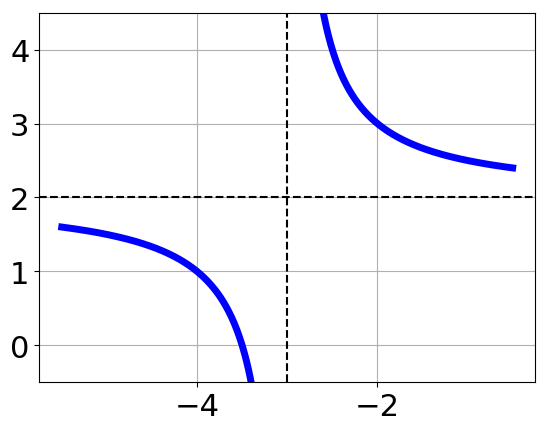
\includegraphics[width = 0.3\textwidth]{../Figures/rationalEquationToGraphAC.png}\item 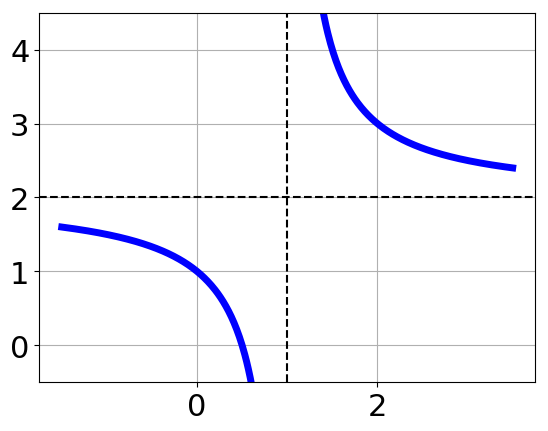
\includegraphics[width = 0.3\textwidth]{../Figures/rationalEquationToGraphBC.png}\item 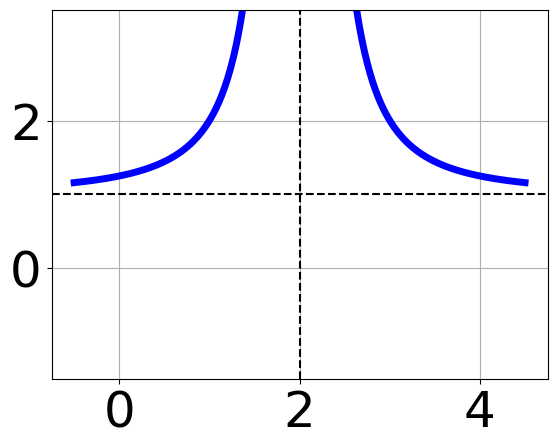
\includegraphics[width = 0.3\textwidth]{../Figures/rationalEquationToGraphCC.png}\item 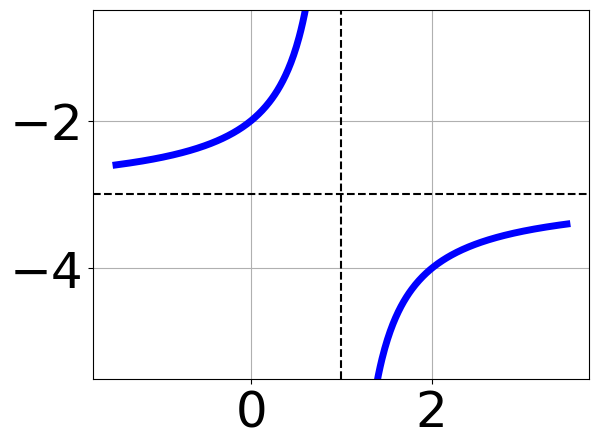
\includegraphics[width = 0.3\textwidth]{../Figures/rationalEquationToGraphDC.png}\end{multicols}\item None of the above.
\end{enumerate} }
\litem{
Solve the rational equation below. Then, choose the interval(s) that the solution(s) belongs to.\[ \frac{-4x}{-7x + 3} + \frac{-3x^{2}}{28x^{2} -61 x + 21} = \frac{-3}{-4x + 7} \]\begin{enumerate}[label=\Alph*.]
\item \( x_1 \in [-2.31, 0.25] \text{ and } x_2 \in [-1.57,2.43] \)
\item \( x \in [3.37,4.36] \)
\item \( x_1 \in [-2.31, 0.25] \text{ and } x_2 \in [0.58,6.58] \)
\item \( \text{All solutions lead to invalid or complex values in the equation.} \)
\item \( x \in [1.34,2.03] \)

\end{enumerate} }
\litem{
Choose the equation of the function graphed below.
\begin{center}
    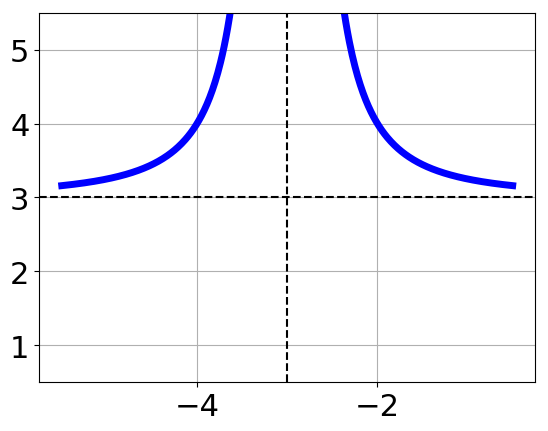
\includegraphics[width=0.5\textwidth]{../Figures/rationalGraphToEquationC.png}
\end{center}
\begin{enumerate}[label=\Alph*.]
\item \( f(x) = \frac{1}{(x - 2)^2} - 3 \)
\item \( f(x) = \frac{-1}{x + 2} - 3 \)
\item \( f(x) = \frac{1}{x - 2} - 3 \)
\item \( f(x) = \frac{-1}{(x + 2)^2} - 3 \)
\item \( \text{None of the above} \)

\end{enumerate} }
\litem{
Choose the graph of the equation below.\[ f(x) = \frac{-1}{x + 2} + 3 \]\begin{enumerate}[label=\Alph*.]
\begin{multicols}{2}\item 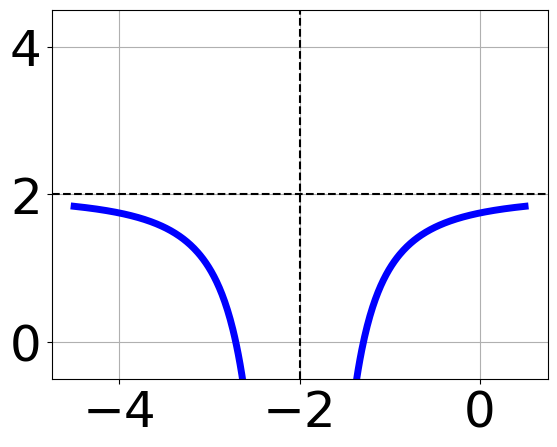
\includegraphics[width = 0.3\textwidth]{../Figures/rationalEquationToGraphCopyAC.png}\item 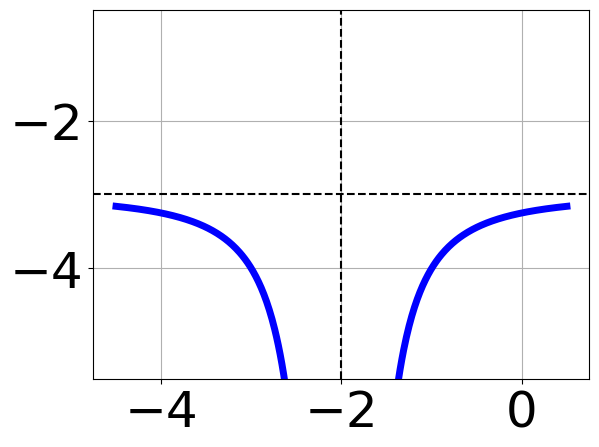
\includegraphics[width = 0.3\textwidth]{../Figures/rationalEquationToGraphCopyBC.png}\item 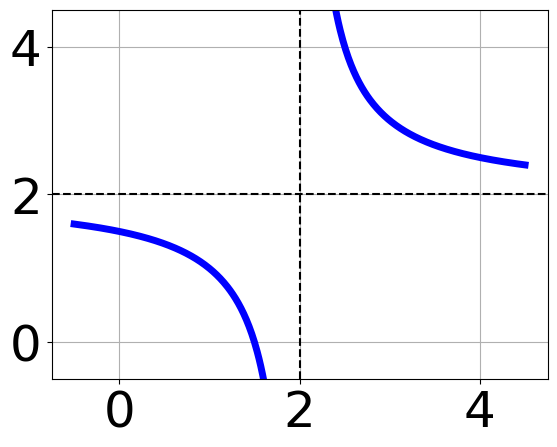
\includegraphics[width = 0.3\textwidth]{../Figures/rationalEquationToGraphCopyCC.png}\item 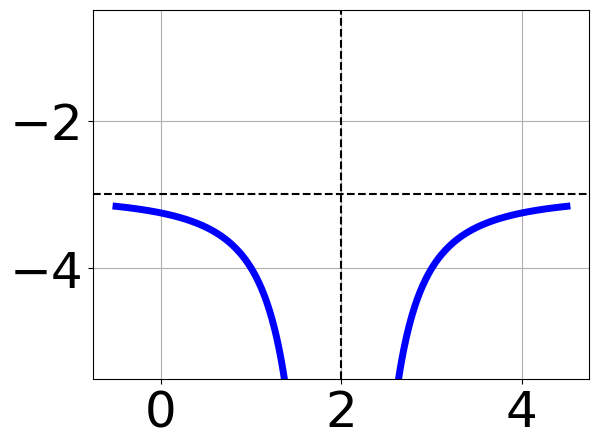
\includegraphics[width = 0.3\textwidth]{../Figures/rationalEquationToGraphCopyDC.png}\end{multicols}\item None of the above.
\end{enumerate} }
\litem{
Choose the equation of the function graphed below.
\begin{center}
    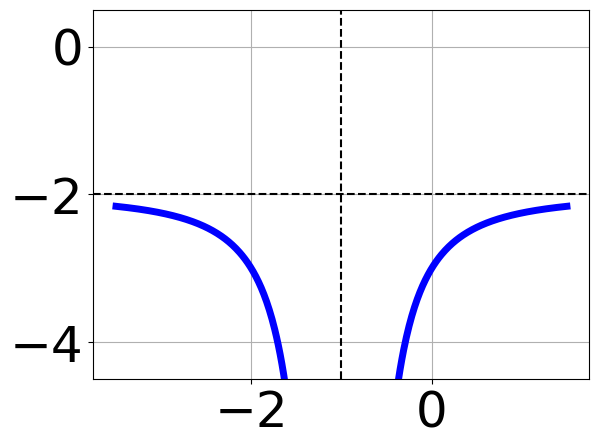
\includegraphics[width=0.5\textwidth]{../Figures/rationalGraphToEquationCopyC.png}
\end{center}
\begin{enumerate}[label=\Alph*.]
\item \( f(x) = \frac{1}{x - 1} + 1 \)
\item \( f(x) = \frac{-1}{(x + 1)^2} + 1 \)
\item \( f(x) = \frac{-1}{x + 1} + 1 \)
\item \( f(x) = \frac{1}{(x - 1)^2} + 1 \)
\item \( \text{None of the above} \)

\end{enumerate} }
\end{enumerate}

\end{document}